\chapter{Background}
\label{background}

\section{Technologies}

There are a number of components needs to build the architecture of a web application. The nature of these components is explored below, and their contribution to the creation of a web application is analysed.

\subsection{Web Application Framework}
The WAF chosen for this project is Spring MVC [Model View Controller]. Shan and Hua defined a WAF as “a defined support structure in which other software applications can be organized and developed”. (Shan and Hua 2006). Model-View-Controller is a software pattern that facilitates the use of a user interface. The Model manages the behaviour and data of the application. The View will manage the information obtained from the model and display it to the user. The Controller takes user input, such as key strokes, mouse movements or a touch display, and can interact and invoke functionality within the Model and/or View.

\begin{figure}[ht!]
\centering
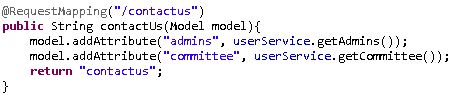
\includegraphics[width=90mm]{figs/fig3-4-1.jpg}
\caption{Contoller adding Model to View}
\label{overflow}
\end{figure}

\subsection{Application Server}

\subsection{Project Management Tool}

\subsection{Database Model}

\subsection{Source Control}

\subsection{Integrated Development Environment}

\subsection{Logging}

\subsection{Web Pages}

\subsubsection{Structure}

\subsubsection{Language}

\section{Usability Studies}

\subsection{Case Study: Monaleen GAA Tennis Club}

\subsection{Case Study: Tralee Tennis Club}